%% Bemærk:
%%          Resten af rapporten følger en stil hvor indledninger skrives
%%          med \sffamlily-typen. Denne stil bør også følges her.
%%
{\sffamily
I denne sektion vil vi test den udvidet løsning, om den virker som vi
hade planlagt på test billeder og om hvordan den virker i praktisk på
udvalgte malerier.
}
\subsection{Afprøvning på testbilleder}
Vi vil teste om den udvidet løsning virker som vi har beskrevet i
opgave, vi ser på 4 test billeder, billedet \ref{hus_virker} er et hus
hvor snittet og massemidtpunktet næsten ligge oven i hinanden. I det
andet billedet \ref{hus_virker_ikke} er huset forskubbet så masse
midtpunktet lige lige uden for margin, og derved ikke skulle blive tage
med af algoritmen. Det tredje billedet har en region som er meget lille
og derfor bliver fra sorteret på grund af den størrelse, den stor
region, bliver taget med at dens massemidtpunkt ligger inden for margin,
denne figur samt huset ville ikke være blevet taget med i den naive
løsning XX(skal jeg overhoved nævne det). Det 4 billedet er der en
region med som har et massemidtpunkt inde i margin, men som har en skæv
fordeling af pixels i forhold til snittet og derfor bliver sorteret fra.
Ud fra de fire observationer, virker den udvidet løsning som vi havde
forventet.

\begin{figure}[!h]
    \centering
		\subfloat[Et hus der er symetrisk og der har massemidtpunkt i spisen af taget, massemidtpunktet er inde for margin så huset bliver udvalgt til at ligge i snittet.]{
        	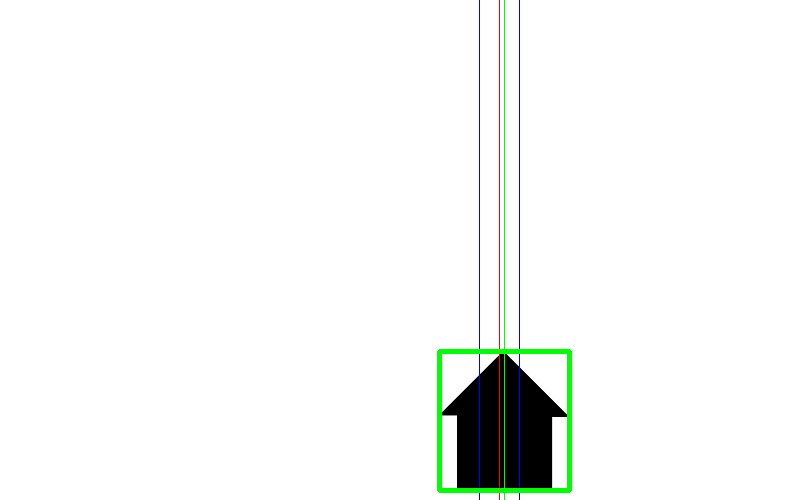
\includegraphics[angle=0,width=1.0\textwidth]{afsnit/afprovning/billeder/udvidet_losning/udvidet_hus1_test.png}
        	\label{hus_virker}}\hspace{1em}
    	\subfloat[Hus hvor masse midtpunktet er flyttet få pixels ud for margin, den udvide løsning vælger ikke at tage huset med]{
        	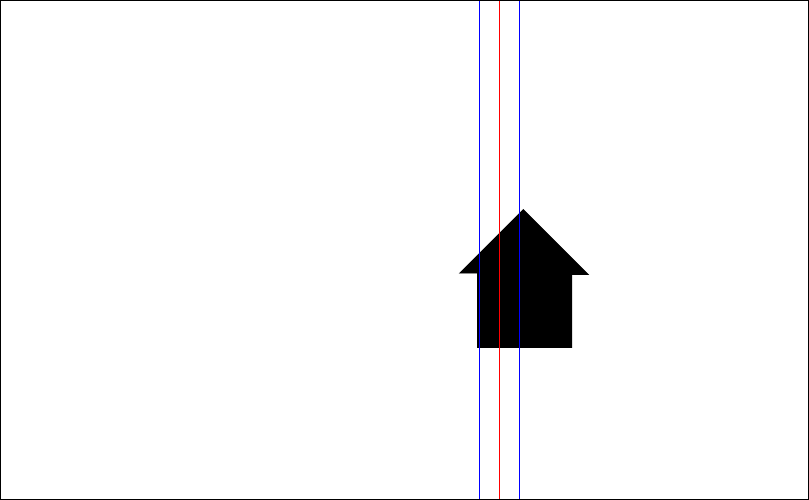
\includegraphics[angle=0,width=1.0\textwidth]{afsnit/afprovning/billeder/udvidet_losning/udvidet_hus2_test.png}
        	\label{hus_virker_ikke}}\hspace{1em}        	    			
        \caption[]{}
     \label{naiv_detektion_test}
\end{figure}

\begin{figure}[!h]
    \centering
    	\subfloat[2 regioner hvor den nederste har et massemidtpunkt inde for margin ]{
        	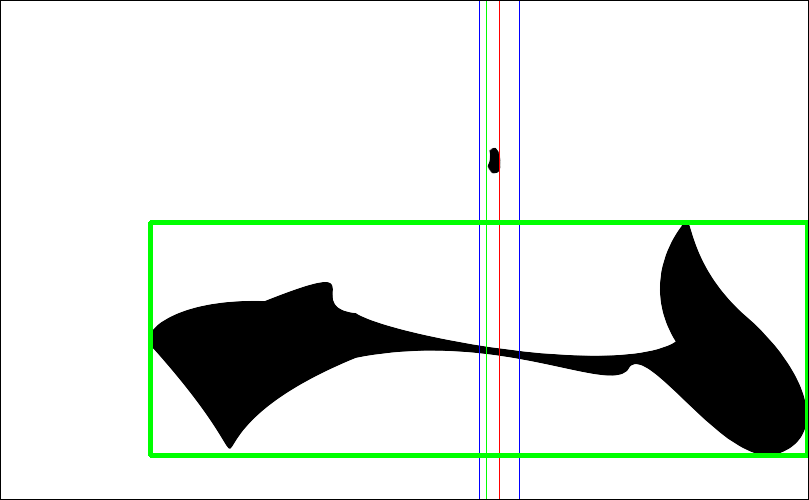
\includegraphics[angle=0,width=1.0\textwidth]{afsnit/afprovning/billeder/udvidet_losning/udvidet_blob2_test.png}
        	\label{udvidet_blob_test}}\hspace{1em}
    	\subfloat[margin er sat meget op, så man kan se at regionen har et massemidtpunkt ind for margin, men da størstedelen af regionens pixels er på højre side, vælger den fra]{
        	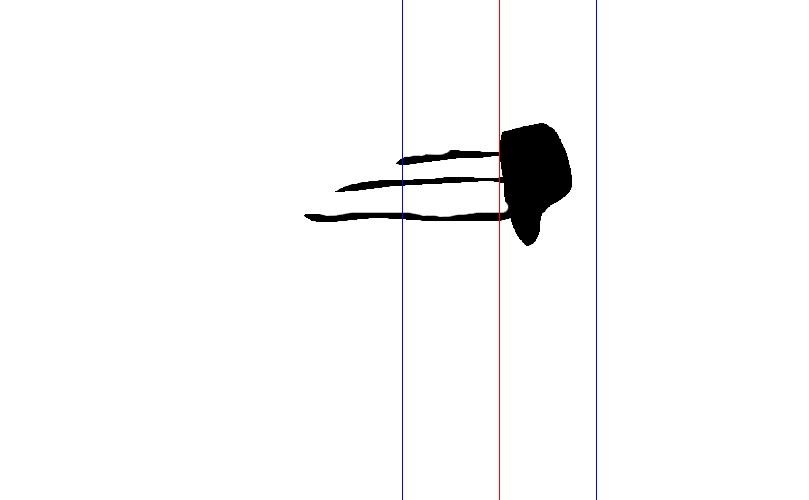
\includegraphics[angle=0,width=1.0\textwidth]{afsnit/afprovning/billeder/udvidet_losning/udvidet_bleksprutte_test.png}
        	\label{bleksprutte_test}}\hspace{1em}        	    			
        \caption[]{}
     \label{naiv_detektion_test}
\end{figure}

\clearpage

\subsection{Afprøvning på malerier}
Afprøvningen af den udvidet løsning på malerier fra vores database vil foregå på samme måde som den naive test. Hvor 6 billeder vil bliver fremvist med en forklaring i deres caption på hvad der sker i billedet og hvorfor.

\begin{figure}[h!!]
	\begin{center}
		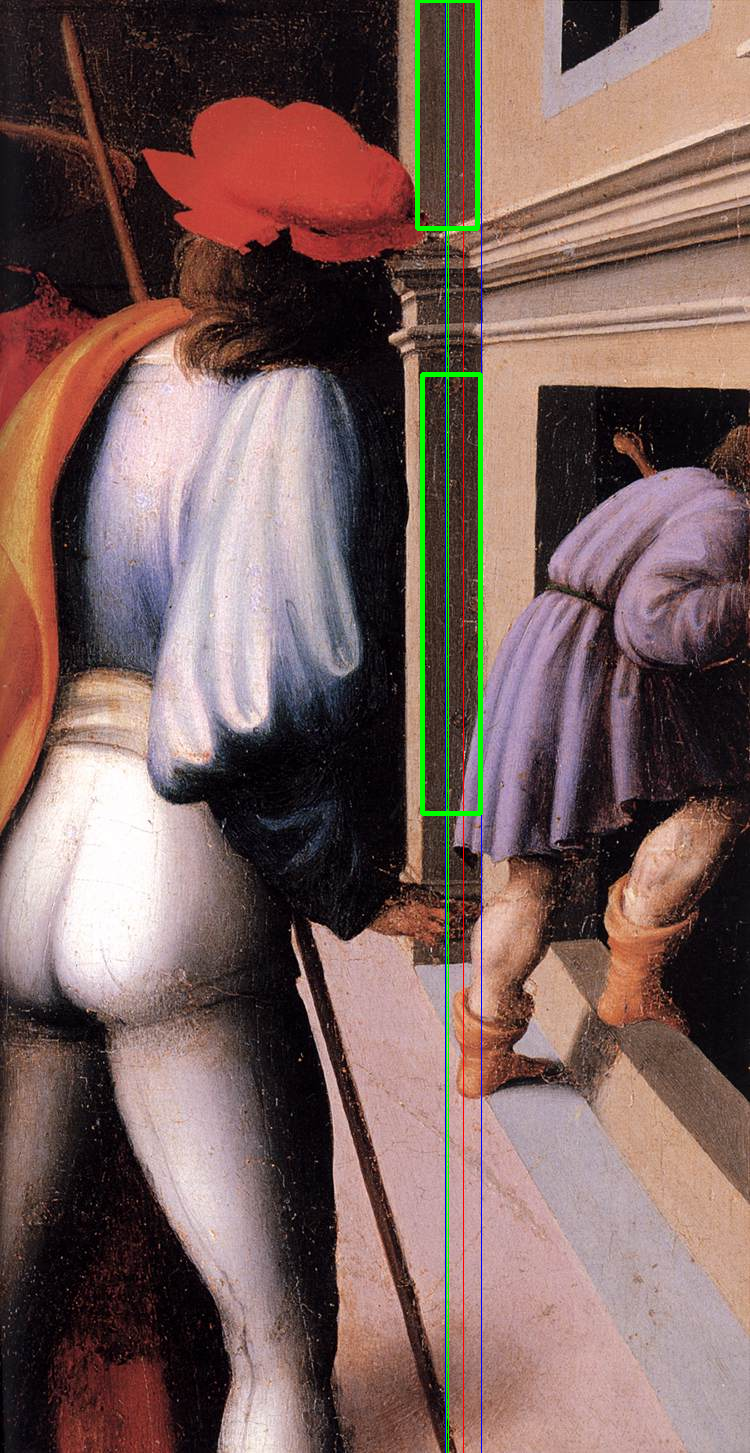
\includegraphics[scale=0.3,angle=0]{afsnit/afprovning/billeder/udvidet_losning/udvidet_kfarver_sdetaljer.png}
	\end{center}
	\caption[]{2 ud af de 6 region er godtager som ligene i det gyldne snit af den udvidet løsning}
	\label{udvidet_virker1}
\end{figure}

\begin{figure}[h!!]
	\begin{center}
		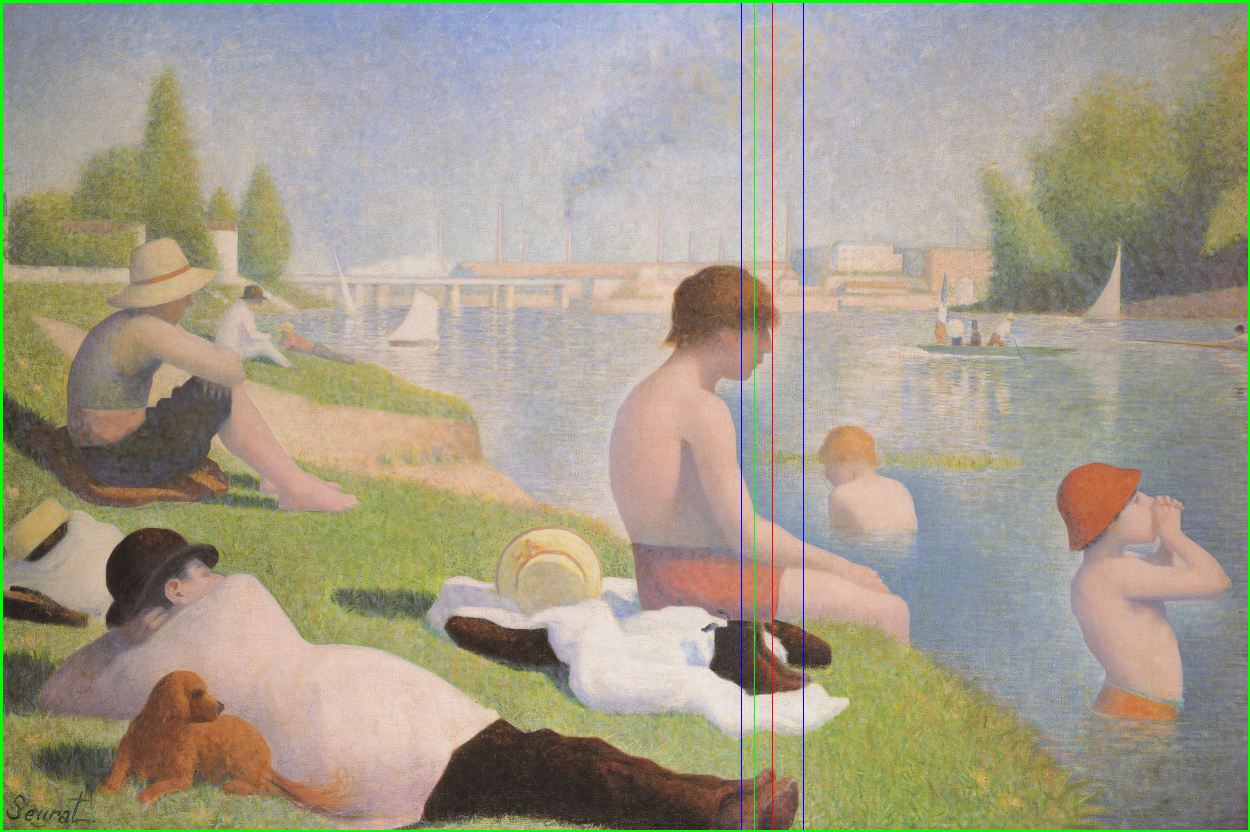
\includegraphics[scale=0.3,angle=0]{afsnit/afprovning/billeder/udvidet_losning/udvidet_dreng.png}
	\end{center}
	\caption[]{baggrunden er den nedeste region som bliver godtaget, da den har et massemidtpunkt som liger inde for marginen}
	\label{udvidet_virker2}
\end{figure}

\begin{figure}[!h]
    \centering
    	\subfloat[Udvidet løsning]{
        	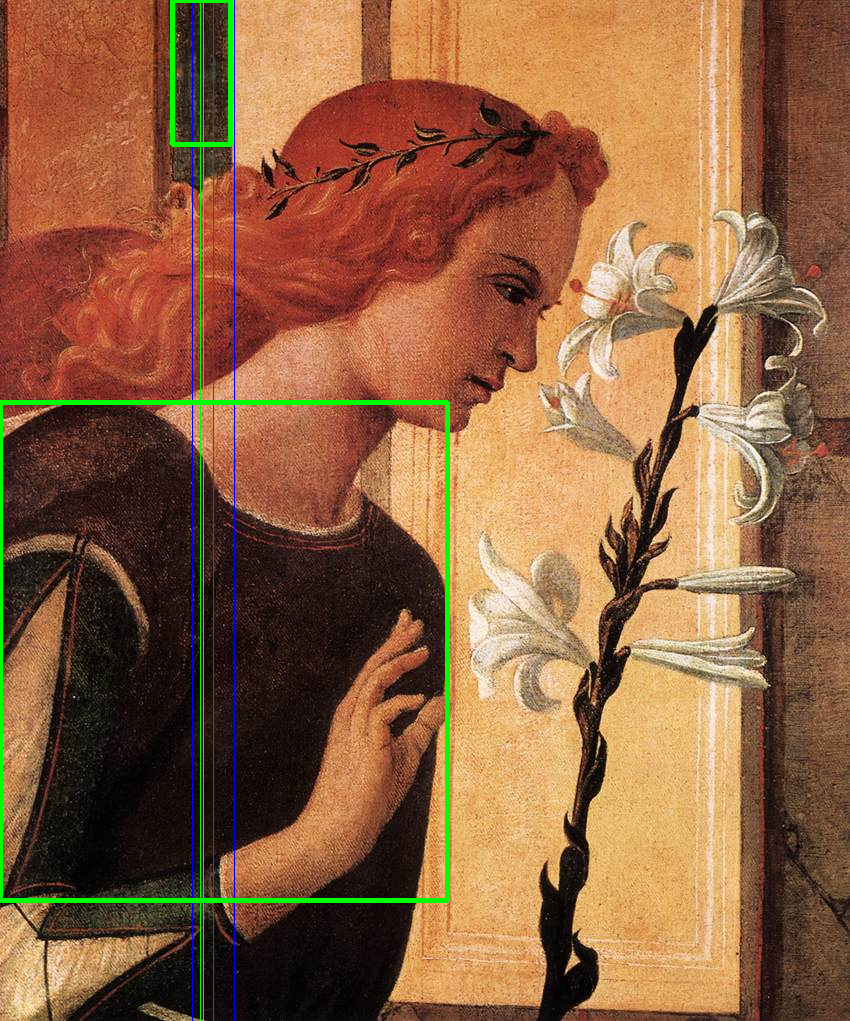
\includegraphics[angle=0,width=0.45\textwidth]{afsnit/afprovning/billeder/udvidet_losning/udvidet_pige.png}
        	\label{udvidet_pige}}\hspace{1em}
    	\subfloat[naiv løsning]{
        	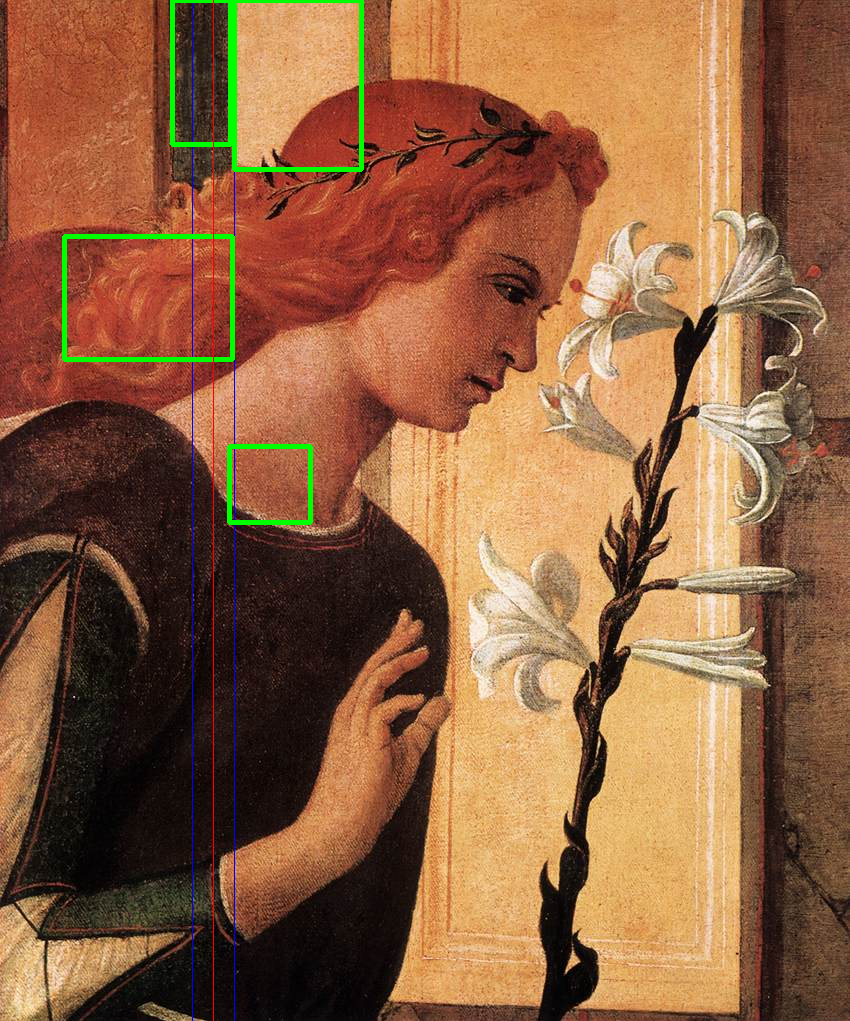
\includegraphics[angle=0,width=0.45\textwidth]{afsnit/afprovning/billeder/udvidet_losning/naiv_pige.png}
        	\label{naiv_pige}}\hspace{1em}        	    			
        \caption[]{Et maleri hvor resultatet for den udvidet og den naive løsning er protrateret. Der bliver fundet forskellige regioner for vær af algoritmerne}
     \label{udvidet_virker3}
\end{figure}

\begin{figure}[h!!]
	\begin{center}
		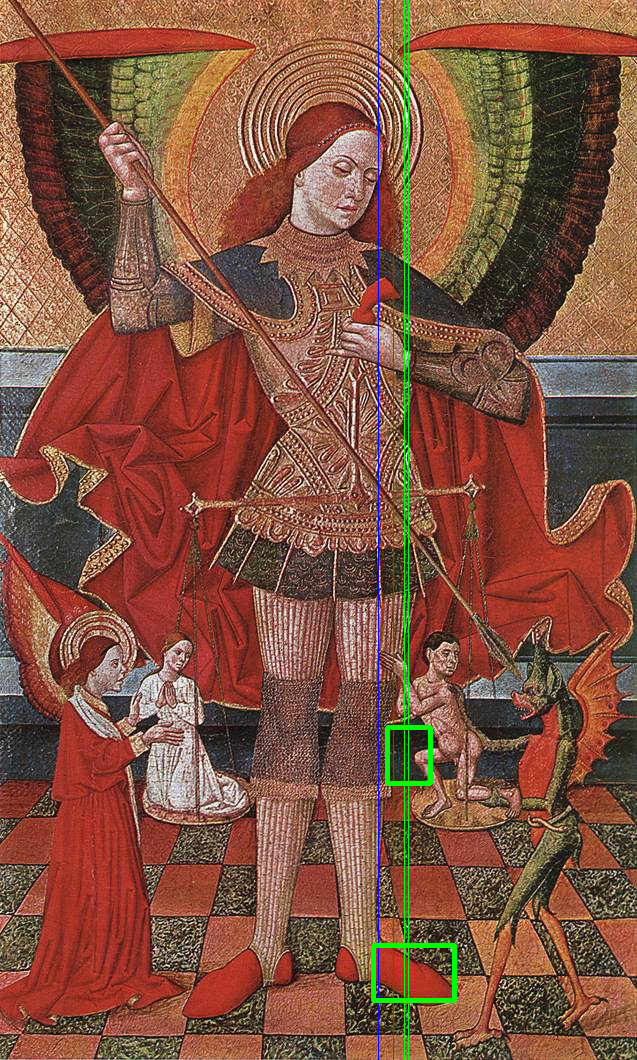
\includegraphics[scale=0.3,angle=0]{afsnit/afprovning/billeder/udvidet_losning/udvidet_kfarver_kdetaljer.png}
	\end{center}
	\caption[]{En sko og en flise bliver taget med at algoritmen}
	\label{udvidet_virker_ikke1}
\end{figure}

\begin{figure}[h!!]
	\begin{center}
		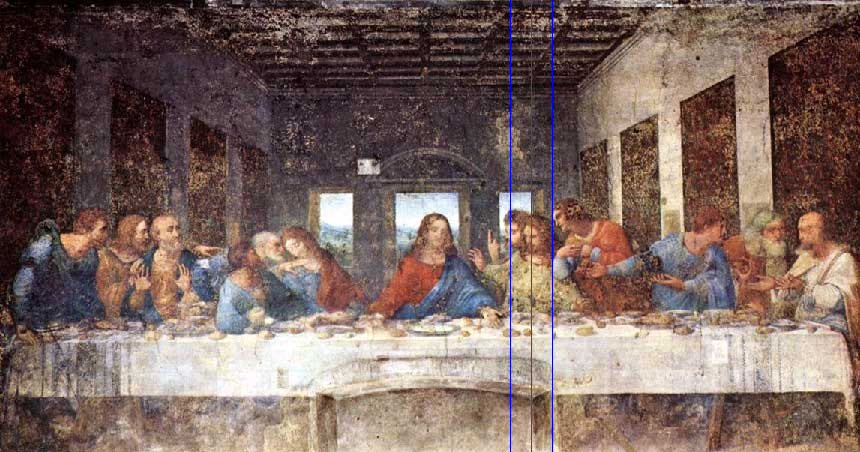
\includegraphics[scale=0.3,angle=0]{afsnit/afprovning/billeder/udvidet_losning/udvidet_mfarver_mdetaljer.png}
	\end{center}
	\caption[]{Den udvidet løsning sortere alle regioner væk}
	\label{udvidet_virker_ikke2}
\end{figure}

\begin{figure}[h!!]
	\begin{center}
		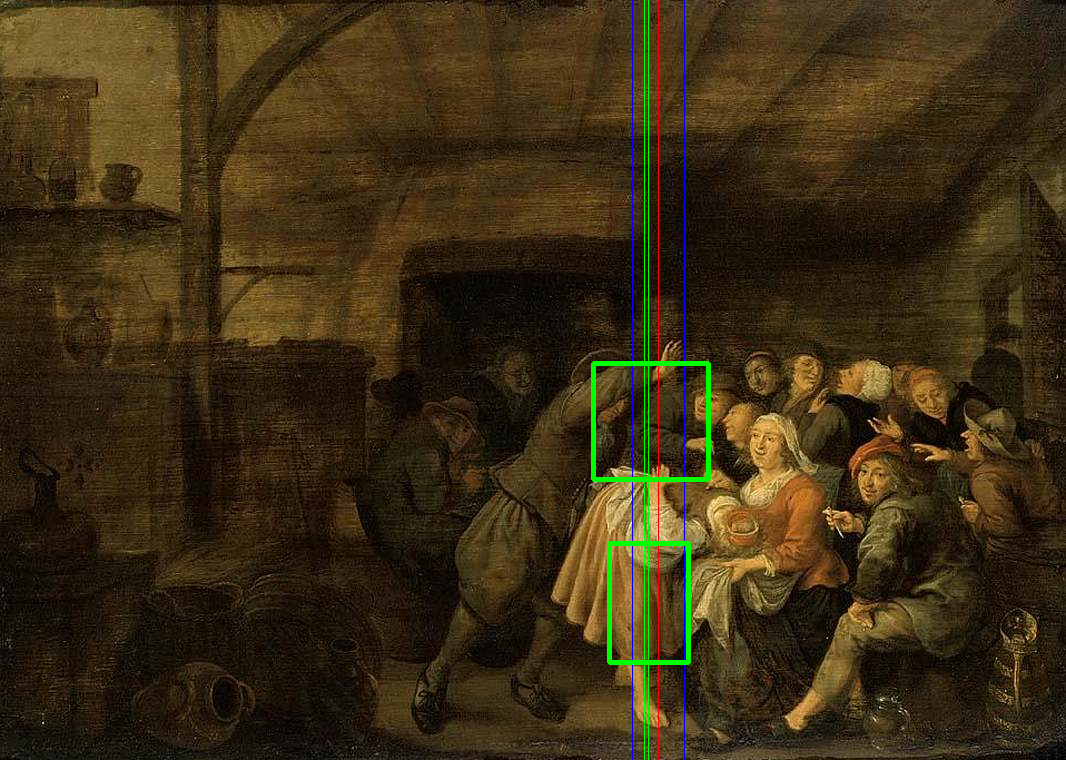
\includegraphics[scale=0.3,angle=0]{afsnit/afprovning/billeder/udvidet_losning/udvidet_sfarver_mdetaljer.png}
	\end{center}
	\caption[]{2 regioner som ikke høre nogle steder hende bliver fundet}
	\label{udvidet_virker_ikke3}
\end{figure}
\clearpage

\subsection{konklution}
Ud for teste billederne ser det ud til at den udvidet metode virker på
den måde som vi havde planlangt at den skulle virke. I den praktiske
brug på malerierne, finder den udvidet løsning mange gode regioner hvis
regions detektoren virker se figur \ref{udvidet_virker1}, men kommer
desværre stadig med få regioner som ikke er særlige gode, f.eks i maleri
\ref{udvidet_virker2}. Der udvidet løsning finder også regioner som den
naive ikke vil finde se en sammenlining i figur \ref{udvidet_virker3}. I
de tilfælde hvor regions detektoren ikke virker godt, er den udvide
løsning god til at sorter regioner væk og kommer derfor ikke med særlige
mange regioner som ikke skulle være der, se figur
\ref{udvidet_virker_ikke2} og \ref{udvidet_virker_ikke3}. Dog kommer vi
stadig ud i problemer hvor der kun er regioner som er forkerte med,
figur \ref{udvidet_virker_ikke1}.
